\documentclass[tikz]{standalone}
\usepackage{tikz}
\usepackage{fontawesome5}
%\usepackage[gray]{xcolor} % Make everything black and white

\begin{document}

\newcommand{\street}[2]{
	\draw[black, line width=2.5mm] (#1) -- (#2);
	\draw[white, line width=0.3mm, dashed]  (#1) -- (#2);
}

\begin{tikzpicture}[x=1mm, y=1mm]

\tikzstyle{vertex} = [circle, draw=black, fill=white, line width=0.5mm]
\tikzstyle{path}   = []

\coordinate (v1) at ( 0, 30);
\coordinate (v2) at (20,  0);
\coordinate (v3) at (40, 30);
\coordinate (v4) at (60,  0);
\coordinate (v5) at (80, 30);

\street{v1}{v2}
\street{v2}{v3}
\street{v2}{v4}
\street{v3}{v4}
\street{v3}{v5}
\street{v4}{v5}

\node[vertex] at (v1) {$1$};
\node[vertex] at (v2) {$2$};
\node[vertex] at (v3) {$3$};
\node[vertex] at (v4) {$4$};
\node[vertex] at (v5) {$5$};

\node at (-6, 31) {\Large \faBuilding};
\node at (86, 31) {\Large \faHome};

\draw[->, red, line width=1.2mm, dash pattern=on 2.8mm off 1.5mm, tension=0.2, smooth] plot coordinates {
  (4,29) (20,6) (35,27) (39, 26) (55,3) (60.5,6) (76,29)
};

\end{tikzpicture}

\end{document}

